\section{Entorno de trabajo}

A continuación describiremos brevemente el entorno de trabajo que hemos empleado para desarrollar el proyecto y que debemos hacer para reproducir este entorno de desarrollo.\par
Hemos trabajado indistintamente sobre sistemas operativos basados en Unix, utilizando Mac OS X y Linux; pero el entorno podría reproducirse para trabajar también sobre Windows.\par
Aunque se trata de un proyecto individual, el código se mantenía bajo un sistema de control de versiones, lo que permite mantener un registro histórico del desarrollo. Mantendremos dos repositorios en Github: uno en el que mantendremos el diseño del framework de Android \cite{meer:android} y otro para desarrollar el generador de código \cite{meer}.\par

\subsection{Python}
La aplicación que genera el código está escrita en Python, así que obviamente necesitaremos el intérprete de Python para poder ejecutarla.\par
Emplearemos la rama 2.x de Python por los motivos que justificamos en el aparado \ref{sec:tecnologias:python}. En las plataformas en las que hemos estado desarrollando podemos encontrar Python en la versión 2.7, la última versión estable del lenguaje, y es sobre esta versión sobre la que trabajaremos.\par

\subsubsection{Pip y VirtualEnv}\label{sec:virtualenv}
Uno de los problemas más comunes en el desarrollo son los conflictos entre librerías y la necesidad de replicar entornos de trabajo.\par 
En Python existen dos herramientas que permiten atajar este problema: pip y virtualenv. \par
Pip es una herramienta para instalar y gestionar paquetes de Python automáticamente. Instalar un paquete con pip es tan sencillo como indicar el nombre del paquete y la versión, como vemos en el ejemplo \ref{pip}.\par

\begin{lstlisting}[language=bash,label=pip,caption=Instalación de un paquete utilizando pip]
	$ pip install SomePackage==1.0  
\end{lstlisting}

También acepta como parámetro para instalar paquetes un fichero las librerías del proyecto, como podemos ver en el ejemplo \ref{pip-req}.\par

\begin{lstlisting}[language=bash,label=pip-req,caption=Instalación de los requisitos de un proyecto utilizando pip]
	$ pip install requirements.txt  
\end{lstlisting}

Para conocer las dependencias de un proyecto únicamente tendremos que ejecutar pip con el parámetro \emph{freeze} y nos devolverá un listado con las librerías que necesita este proyecto, que guardaremos en un fichero requirements.txt, lo que nos permitirá replicar el entrono fácilmente. \par
En esta aplicación únicamente hacemos uso de la librería externa Jinja2, y esta a su vez necesita MarkupSafe y wsgiref. Así que el fichero con los requisitos será como el que vemos en la \ref{requisitos}.\par

\begin{lstlisting}[language=bash,label=requisitos,caption=Requisitos del proyecto]
	Jinja2==2.7
	MarkupSafe==0.18
	wsgiref==0.1.2
\end{lstlisting}


La otra herramienta de la que haremos uso es virtualenv  que  crea entornos virtuales de Python aislados evitando los conflictos de dependencias entre las librerías de un proyecto y permite replicar el entorno fácilmente.\par
Cada entrono virtual contiene su propia versión de Pip encapsuladas. Lo que permite instalar librerías dentro del entorno que hayamos creado.\medskip\par

La combinación de estos dos paquetes nos permite tener entornos de trabajo con todas las dependencias del proyecto que pueden ser replicados con facilidad. 

\subsection{Android}

Tanto para desarrollar el prototipo como para crear el framework de Android que instanciará los informes DICOM-SR, necesitamos trabajar dentro del entorno de desarrollo de Android.\par
Para desarrollar una aplicación haremos uso de las siguientes herramientas:
\begin{itemize}
\item El kit de desarrollo de Java (JDK).	
\item La kit de desarrollo de  Android (Android SDK). En nuestro caso necesitaremos la SDK de la versión 3.2.
\item El IDE de desarrollo Eclipse.
\item El plugin para Eclipse para poder trabajar con Android. (ADT)
\end{itemize}

\medskip\par
Concluyendo, tenemos un entrono de trabajo para el generador de código y otro para el desarrollo de la aplicación framework de Android. Esto nos permite desarrollar de modo independiente cada una de las partes que componen la arquitectura de la solución.


\section{Aplicación framework de Android}
El desarrollo de la solución final sigue la metodología en cascada. Pero necesitamos desarrollar simultáneamente una aplicación Android que nos servirá como esqueleto (o framework) para insertar en ella el código que generemos a partir de un informe DICOM-SR concreto.\par 
Para esta aplicación Android necesitamos que el usuario valide las decisiones de diseño e interacción que hemos tomado, por lo tanto ya durante la etapa de diseño elaboramos un prototipo como ya hemos explicado en el apartado \ref{prototipo}.\par

Este mismo prototipo lo haremos evolucionas para que nos sirva como esqueleto para las aplicaciones generadas. Simplemente eliminaremos del prototipo todas las partes que correspondan a un informe concreto, y las sustituiremos por el código generado automáticamente. Y añadiremos las funcionalidades que sean genéricas para todas las aplicaciones que se generan a partir de informes DICOM-SR. \medskip\par

Durante el desarrollo de este prototipo nos dimos cuenta que algunas de las pantallas diseñadas en la etapa anterior no podían generalizarse fácilmente. Por ejemplo, en las figuras  \ref{fig:mockup:tree} y \ref{fig:mockup:treenodes}  veíamos todas las posibles lesiones de todos los órganos de este informe como no siempre habrán dos órnagos involucrados en un informe, esta pantalla no podía generalizarse.\par
Decidimos entoces ordenar las pantallas siguiendo la estructura propia del informe. Si bien la solución propuesta en el apartado \ref{sec:ui-mockup} agrupa el conocimiento de una forma algo más simple para el usuario final que únicamente sirva para un subconjunto de informes médicos hace que la descartemos. Optando por una solución genérica que permita transformar en una aplicación Android cualquier plantilla de informe médico.\medskip\par  

Para no duplicar información, podremos ver las modificaciones realizadas en la aplicación esqueleto en el apartado \ref{sec:appfinal}.\par
Resumiendo hemos evolucionado el prototipo desarrollado en la etapa anterior para poder instanciar todo tipo de infores médicos. De esta aplicación Android, eliminamos los fragmentos que pertenecen a un informe concreto quedándonos el esqueleto que después completaremos con el código generado automáticamente. 


\section{Analizador sintáctico}
El análisis sintáctico (parsing) se encarga de leer el fichero de tipo DICOM-SR y crear una estructura de datos en memoria con la información del fichero. La estructura de datos más comúnmente empleada para esta tarea es un  árbol ya que encapsula la información tanto de los nodos como de la jerarquía.\medskip\par

Los analizadores sintácticos de XML se dividen en dos categorías fundamentalmente \cite{li2009xml}: analizadores DOM (Document Object Model) y SAX (Simple API for XML).\par
DOM emplea es una interfaz de aplicación (API) basada en árbol que modela todo el documento XML como un árbol. Es adecuado cuando queremos realizar operaciones sobre ficheros complejos y sobre los que realizan accesos aleatorios, porque en el árbol generado tenemos toda la información del informe. Pero este árbol que genera puede llegar a ser hasta 10 veces más grande que el fichero XML lo hace poco apropiado para tratar con ficheros grandes.\par
SAX, por el contrario es una interfaz de aplicación basada en eventos. Lee el fichero secuencialmente, cada nodo leído provocará que se lance un evento que es tratado por el analizador de tipo SAX. SAX es apropiado para ficheros grandes, porque según va leyendo el fichero lanzará los eventos asociados y descarta la información de lo leído hasta este punto. Su complejidad espacial es menor porque no necesita almacenar mucha información en memoria. Precisamente por este motivo no permite realizar operaciones que requieran de información global.\par
En nuestro caso, los informes DICOM-SR con los que trabajamos son potencialmente muy largos, por lo que un análisis tipo DOM queda descartado. Sin embargo, para generar el código necesitaremos un árbol, lo que haremos tras el análisis es generar una estructurea arbórea eficiente. Este proceso se describe en el apartado \ref{sec:better_tree}.\medskip\par

En la librería estándar de Python podemos encontrar el paquete \emph{xml.sax}, que implementa la interfaz de SAX.\par
Como en nuestro caso queremos extender el comportamiento del analizador sintáctico XML para que sea capaz de interpretar ficheros con plantillas de informes médicos DICOM-SR, por lo tanto crearemos una clase que extienda de la clase \emph{xml.sax.ContentHandler} que es precisamente la clase que trata los eventos lanzados por el analizador sintáctico.\medskip\par

En la figura \ref{fig:uml-parser} hemos visto el diagrama UML que modela esta clase.\par
Los atributos internos nos permiten almacenar información acerca de lo leído en el fichero y al terminar el análisis generar un árbol con los datos del informe DICOM-SR.\par

En el segmento de código \ref{DicomParser} vemos como la clase \emph{DicomPasrser} extiende del analizador sintáctico SAX estándar. Recibe un informe DICOM-SR que sigue el formato XML y en la variable interna \emph{self.\_dict\_report} devolverá la estructura arbórea eficiente con la información del fichero DICOM-SR.\par

\lstset{escapechar=@,style=python}
\begin{lstlisting}[label=DicomParser,caption=Clase que analiza sintácticamente un fichero DICOM-SR]

class DicomParser(xml.sax.handler.ContentHandler):
    
    ...

    def parse(self, xml_file):
        """ Parse the file using this handler.
        Returns the report using a DictReporT.

        Keyword Argument:
        xml_file  -- XML file in DICOM format to parse

        """
        xml.sax.parse(xml_file, self)
        return self._dict_report

\end{lstlisting}

Los métodos que hemos sobrecargado para recoger información del informe DICOM-SR son los siguientes:
\begin{itemize}
\item \emph{startElement}: es llamado cada vez que un nueva etiqueta de apertura de un nodo. En nuestro caso lo empleamos para iniciar variables y preparar las variables que nos indican en que punto del análisis sintáctico nos encontramos.
\item \emph{endElement}: se llama cuando se encuentra un final de etiqueta. Si se trata del final de un atributo, almacenamos la información en un contenedor temporal de tipo \emph{SAXContainer} y si se trata del final del contenedor en si, lo añadimos a la variable interna de tipo \emph{SAXReport} que guarda una lista con todos los contenedores DICOM-SR encontrados. 
\item \emph{characters}: se llama cada vez que se lee un carácter y este es almacenado en un buffer.
\item \emph{endDocument}: finalmente cuando termina el documento se llama este método. Como en este punto ya tenemos toda la información del fichero, la reorganizaremos en forma de árbol. Este proceso lo explicaremos en el apartado \ref{sec:better_tree}.
\end{itemize}\medskip\par

En los informes DICOM-SR, cada contenedor sigue un formato estándar lo que le da gran versatilidad. En un contenedor DICOM-SR sus atributos y los contenedores que cuelgan de este contenedor se agrupan bajo la etiqueta de los hijos.Por simplicidad para generar el código, hemos agrupado los atributos dentro del contenedor y sus hijos serán únicamente otros contenedores.\par
En la figura \ref{fig:SAXReport_schema} vemos un esquema de cómo se estructura la información en el analizador sintáctico, al compararla figura \ref{fig:dicom-report} encontramos las diferencias que hemos descrito respecto a un fichero DICOM-SR.\par

\begin{figure}[ht]
\centering
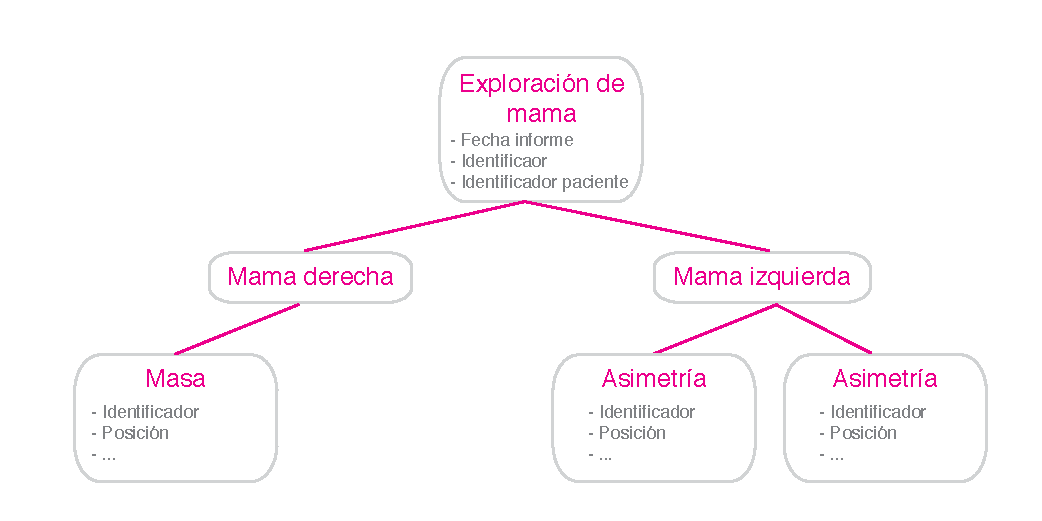
\includegraphics[scale=0.7]{./imgs/esquemas/dicomsrTreeSAX.pdf}
\caption{Esquqema del árbol DICOM-SR para el analizador sintáctico}
\label{fig:SAXReport_schema}
\end{figure}


Para almacenar la información a medida que vamos leyendo creamos dos clases: \emph{SAXContainer} y \emph{SAXReport}.\par
En el segmento de código \ref{SAXContainer} vemos la interfaz de la clase desarrollada para almacenar y gestionar los contenedores DICOM-SR mientras se está leyendo el fichero. Como ya hemos explicado los atributos DICOM-SR se integran dentro del contenedor. Además hemos definido atributos como \emph{open}, \emph{parent} y \emph{tree\_level} para almacenar elementos de la estructura del informe que nos permitirán después construir el árbol.\par

\begin{lstlisting}[label=SAXContainer,caption=Clase que almacena información durante el análisis de un contenedor]

class SAXContainer(object):
    """This class stores a container tag from xml"""
    def __init__(self, concept=Concept(), level=-1, 
    			 open_level=True, parent=Concept(),
    			 properties=Property()):
        self.concept = Concept(concept.value, concept.schema, concept.meaning)
        #A list of attributes/nodes (date, num, text)
        self.attributes = []
        self.tree_level = level
        self.open = open_level
        self.parent = parent
        self.properties = properties

    def has_concept(self)

    def add_attribute(self, attribute)

	def __repr__(self)
\end{lstlisting}

Dentro de cada contenedor se almacena un concepto DICOM-SR. Son los conceptos los que mantiene la información en si del sistema. Tenemos la clase \emph{Concept} y \emph{Data type} con sus hijos para cada tipo de dato que pueda aparecer en el informe \emph{Num} (números), \emph{Text} (cadenas de texto), \emph{Code} (cadenas de texto de un conjunto de posibilidades) y \emph{Date} (fechas). Hemos visto el diagrama UML en \ref{fig:uml-types}.\medskip\par


En \ref{SAXReport} vemos la interfaz  de la clase que almacenará el informe durante el análisis sintáctico del informe. Mantiene informcación de la ontología a la que pertenece el informe médico y una lista con los contenedores DICOM que vamos leyendo.\par

\begin{lstlisting}[label=SAXReport,caption=Clase que almacena información durante el análisis de un informe]

class SAXReport(object):
    """This class manages the report while we are reading it from xml"""
    def __init__(self):
        self.report_type = ""
        self.id_odontology = -1
        self._containers = []

    def add_attribute(self, child_level, current_attribute)

    def add_container(self, new_container)

    def close_level(self, child_level)

    def return_parent(self, tree_level)
	
	def __repr__(self)
\end{lstlisting}

Al finalizar en análisis sintáctico tendremos una lista con todos los nodos del informe.\par 
Aunque en algún caso de traductor orientado a la sintaxis tras el análisis se genera directamente el código, en nuestro caso antes construiremos un árbol con la información leída. La complejidad que añadimos en este paso adicional después simplificará la generación de código, que es el punto más importante de esta aplicación.\par


\section[Árbol DICOM-SR]{Estructura de datos para almacenar un informe DICOM-SR%
              \sectionmark{Árbol DICOM-SR}}
\sectionmark{Árbol DICOM-SR}\label{sec:better_tree}
Antes de adentrarnos en la estructura árborea que hemos diseñado justificaremos su idoneidad para este proyecto.\par
Con este objetivo desarrollamos un sistema de pruebas que generaba las aplicaciones de un conjunto de informes DICOM-SR utilizando el informe almacenado dentro de una lista y con el árbol. Hemos calculado la media del tiempo de usuario empleado para generar un informe. Podemos ver los resultados de generar únicamente la interfaz de usuario en la tabla \ref{table:tiempos1} y en la tabla \ref{table:tiempos2} vemos el tiempo empleado en generar completamente la aplicación Android.\par


\begin{table}[ht]
\begin{minipage}[b]{0.45\linewidth}\centering
\begin{tabular}{c|c|c}
 \hline
 \cellcolor{RubineRed} {\color{White} \backslashbox{Nº informes}{EDA}}  & Lista & Árbol  \\
 \hline
10 & 0.476 s. & 0.51 s \\
 \hline
100 & 0.48 s. & 0.545 s.\\
 \hline
1000 & 0.464 s. & 0.521 s. \\
\hline
\end{tabular}
\caption{Tiempos de ejecución para la generación de la interfaz de usuario}
\label{table:tiempos1}
\end{minipage}
\hspace{0.5cm}
\hfill
\begin{minipage}[b]{0.45\linewidth}
\centering
\begin{tabular}{c|c|c}
 \hline
 \cellcolor{RubineRed} {\color{White} \backslashbox{Nº informes}{EDA}}  & Lista & Árbol  \\
 \hline
10 & 0.92 s. & 0.812 s. \\
 \hline
100 & 0.97 s. & 0.801 s. \\
 \hline
1000 & 0.956 s. & 0.795 s. \\
\hline
\end{tabular}
\caption{Tiempos de ejecución para la aplicación Android}
\label{table:tiempos2}
\end{minipage}
\end{table}

Lo que observamos a partir de estas tablas es que cuando generamos la interfaz de usuario o siendo más generalistas secciones del código que necesitan recorrer todo el informe y que no tienen en cuenta la jerarquía de los nodos, el código que utiliza una lista es más rápido porque no hemos necesitado emplear recursos en crear un árbol con el informe. En cambio si tenemos que generar toda la aplicación, lo que implica segmentos de código que necesitan información jerárquica, el tiempo utilizado en crear el árbol se compensa al generar el código.\par

Los informes que hemos empleado en el script para calcular los tiempos eran de tamaño medio y pequeño. Si utilizamos informes más grandes los resultados serían más abultados, pero en definitiva el uso de un árbol para generar el código está justificado.\medskip\par

En la librería estándar de Python no exista una estructura de árbol, así que nos declaramos una clase para árboles que pueda almacenar cualquier tipo de valor. La interfaz de esta clase podemos verla en \ref{defaultTree}.\par
Es un árbol sobre el que se implementan métodos típicos como: recorridos en profundidad y anchura, búsqueda, vaciado, añadir nuevos elementos y la impresión en forma de árbol. Y otros métodos orientados a la tarea para la que vamos a utilizar este árbol como: \emph{get\_set\_data} que devuelve un conjunto de nodos sin elementos repetidos, \emph{get\_flat\_tree} que devuelve el árbol aplanado dentro de una tabla hash o \emph{get\_code\_containers} que nos devuelve una lista con los identificadores de los elementos de árbol de tipo ``CODE''.\par 

\begin{lstlisting}[label=defaultTree,caption=Clase para árboles genéricos]

class Tree():
    """Tree Object, contains value and child references"""
    def __init__(self, value=None, children=None):
        self.value = value
        if children is None:
            self.children = []
        else:
            self.children = children

    def breadthFirst(self)

    def depthFirst(self)

    def __contains__(self, item)

    def clear(self)
    
    def get_set_data(self,containers,attributes)

    def is_leaf(self)

    def print_tree(self,ident)

    def add_node(self, container, parent)

    def get_flat_tree(self,flat)

    def get_code_containers(self)

\end{lstlisting}

En este árbol los nodos almacenarán la información de un Contenedor DICOM-SR, para esto hemos definido una clase de tipo \emph{Container}. La interfaz de esta clase la podemos ver en \ref{container}. Se trata de una clase muy similar a \ref{SAXContainer}, pero como en este punto ya no necesitamos información acerca de la jerarquía del informe porque esta información se conserva en la estructura del árbol, ni necesitamos información acerca del estado del análisis sintáctico porque ya lo hemos completado, descartamos estos atributos para así aligerar la estructura de datos en la medida de lo posible.\par

\begin{lstlisting}[label=container,caption=Clase para contenedores DICOM-SR]

class Container(object):
    def __init__(self, tree_level, concept=Concept(), 
    			 properties=Property(), attributes=[]):
        self.tree_level = tree_level
        self.concept = concept
        self.properties = properties
        self.attributes = attributes[:]

    def get_code(self)

    def get_schema(self)

    def get_meaning(self)

    def get_level(self)

    def get_concept(self)

    def get_schema_code(self,sep='_')

    def has_code(self,code)

    def __str__(self)

    def __repr__(self)

\end{lstlisting}

Finalmente nos queda ver como se integra el árbol en la clase que modela el informe DICOM-SR.\par
Como vemos en \ref{dicomSRcode}, la interfaz de esta clase es análoga a la definida en \ref{SAXReport}, descartando la información que ya no es necesaria y encapsulando los contenedores del informe dentro de un árbol en lugar de en una lista.\par

\begin{lstlisting}[label=dicomSRcode,caption=Clase para contenedores DICOM-SR]

class DicomSR(object):
    def __init__(self, report_type="", id_ontology=-1):
        self.report_type = report_type
        self.id_ontology = id_ontology
        self.report = Tree()

    def __repr__(self)

    def add_node(self, node, parent):

    def get_ontology(self):

    def get_flat_data(self):

    def get_root(self):

    def get_data_form_report(self, languages, template_type):

\end{lstlisting}

La transformación de una estructura de datos en otra se realiza al finalizar en análisis sintáctico. \par
Cuando el analizador sintácico SAX alcance el final del documento, lanzará un evento \emph{endDocument} y en este punto construiremos el árbol. \par
En \ref{build_dicom_tree}, vemos como hemos construido este árbol. Primero ordenamos los contenedores de la lista y vamos recorriendo esta lista ordenada insertándolos en su posición correcta en el árbol. \par

\begin{lstlisting}[label=build_dicom_tree,caption=Constructor de un árbol DICOM-SR]

    def build_dicom_tree(self):
        """ Build a DicomSR tree using the information read in the file."""
        self._dict_report = DicomSR(self._report.report_type,
                                    self._report.id_odontology)
        #Sort containers list by its tree level.
        self._report._containers.sort(key=lambda x: x.tree_level)
        for container in self._report._containers:
            self._dict_report.add_node(
                Container(container.tree_level, 
                		  container.concept,
                          container.properties,
                          container.attributes),
                container.parent)
\end{lstlisting}

Aunque generar el árbol y rellenarlo suponga añadir una etapa más a la generación de código. Este paso intermedio simplifica el proceso de generaración automática de código, especialmente de aquellas partes de código que necesiten información jerárquica del informe médico.\par

\section{Generador de la aplicación Android}
Tras la etapa anterior tenemos el informe DICOM-SR cargado en memoria en una estructura de árbool. La siguiente etapa será la de generar el código necesario para instanciar la aplicación Android framework para un informe DICOM-SR concreto.\par

\subsection{Configuración}\label{sec:configuracion}
Un generador de código no necesita de la intervención del usuario, de hecho cuanto más automatizado esté el proceso más efectivo será.\par
Sin embargo existen ciertas opciones que permitimos que el usuario configure, como son: la ruta o el nombre de cada nivel jerárquico del informe DICOM-SR en función de la ontología. \par
Además ciertas funciones internas como la ruta en la que se encuentran las plantillas para cada elemento, la internacionalización, \ldots también se establecen utilizando ficheros de codificación.\medskip\par
La librería estándar de Python nos ofrece un módulo para gestionar la configuración de manera muy simple, se trata de \emph{ConfigParser}.\par
Este módulo nos permitirá leer tanto la configuración establecida por el  usuario como la establecida por el sistema.\par
Los ficheros que utiliza \emph{ConfigParser} estructuran la información mediante secciones, que se indican ente corchetes [ ]. Cada sección almacena los datos de configuración mediante pares clave-valor.\par
En \ref{settingsINI} vemos un ejemplo de configuración con la sección que contiene la ruta dónde se almacenará el código generado. La sección es \emph{[Output Directories]} y como podemos ver los ficheros de configuración permiten interpolar valores; por ejemplo: el directorio dónde se guardarán las actividades es el siguiente: \emph{Activities: \%(MainDir)s/activities}, cuando preguntemos a \emph{ConfigParser} por este valor nos devolverá la siguiente ruta: \emph{./outputs/activities}.\par

\begin{lstlisting}[label=settingsINI,caption=Sección del fichero de configuración]
...

[Output Directories]
MainDir: ./outputs
Strings: %(MainDir)s/strings
Activities: %(MainDir)s/activities
Model: %(MainDir)s/models
Layouts:  %(MainDir)s/layouts
Logs: ./logs
Parser: %(Logs)s/parser.log
Properties: ./templates/properties
Manifest: %(MainDir)s/manifest

...
\end{lstlisting}

La gestión de estos ficheros de configuración ha hacemos dentro del módulo \emph{core}. Puesto que necesitaremos acceder a la configuración desde distintos módulos del programa y por lo tanto tiene sentido que este módulo este accesible.\par
El fichero \emph{config.py} contiene las funciones que tratarán con los ficheros de configuración, así como la gestión de otros aspectos de la configuración como la interacionalización. Las funciones más relevantes para este propósito son las siguientes:
\begin{itemize}
\item \emph{set\_environment}: establece las variables de entorno de Jinja para la gestión de plantillas. Hablaremos más en profundidad de este tema en \ref{sec:jinja}.
\item \emph{get\_languages}: devuelve una lista con los idiomas soportados por la plantilla.
\item \emph{read\_config}: crea una instancia de \emph{ConfigParser} y lee el ficheros con la configuración.
\item \emph{get\_filepath}: devuelve la ruta dónde debemos generar los ficheros de un tipo concreto.
\item \emph{get\_filename}: instancia el nombre del fichero con los datos concretos del informe
\item \emph{get\_property}: devuelve una propiedad concreta del fichero de configuración. 
\item \emph{get\_substitution\_options}: devuelve todas las opciones de una sección del fichero de configuración.
\item \emph{get\_language\_code}: devuelve el código del idioma asociado a la etiqueta del informe DICOM-SR. Utilizamos esta funcionalidad para generar las cadenas de texto internacionalizadas. En el apartado \ref{vista:strings} explicaremos esto con más detalles.
\item \emph{get\_ontology\_level}: Devuelve el nombre de un nivel del árbol DICOM-SR basándose e la ontología.
\item \emph{get\_substitution\_dictionary}: devuelve un diccionario con las cadenas listas para internacionalizar las plantillas. 
\item \emph{get\_layout\_settings}: cada nivel del árbol se puede configurar tiene ciertas opciones configurables en la interfaz como por ejemplo si los datos se distribuirán en 1 o 2 columnas. Esta función nos devuelve las opciones de configuración para un nivel de una ontología.
\end{itemize}
Todas estas funciones, junto con los ficheros de configuración, permiten parametrizar y adaptar la aplicación que generemos a las necesidades del usuario. Además al centralizar la gestión de la configuración evitamos tener código repetido en cada uno de los módulos de la aplicación.\par

\subsection{Plantillas}\label{sec:templates}
\subsubsection{String.Template}
\subsubsection{Jinja}\label{sec:jinja}

\subsection{Generador del modelo}\label{sec:generacion}
\subsection{Generador de la vista}
\subsubsection{Generador de la interfaz de usuario}
\subsubsection{Generador de las cadenas de texto}\label{vista:strings}

\subsection{Generador del controlador}
\subsubsection{Generador de las actividades}

%\section{Generador de la plantilla de resultados}
